\chapter{Implementación} \label{ich:implementacion}

Las nuevas técnicas que introducimos implican un esfuerzo considerable en la implementación de módulos de código. Como comentamos en \customref{isubsubs:observaciones_conclusiones_pksampling}, el uso de \textit{P-K sampling} provoca que no podamos usar librerías de aprendizaje automático para realizar tareas comunes, como muestreo de datos, funciones de pérdida, métricas, \ldots

Por tanto, en esta sección explicaremos todo el trabajo de implementación realizado.

\section{Control de versiones y buenas prácticas} \label{isec:github_buenas_practicas}

Para el control de versiones, usamos \textit{Git} con \textit{Github}. Todo el desarrollo del trabajo, tanto la implementación de código como la escritura de la presente memoria, se ha realizado en un repositorio abierto alojado en \cite{informatica:repogithub}.

Gracias al uso de \textit{Github} hemos podido implementar fácilmente una serie de buenas prácticas de desarrollo, entre las cuales se encuentran:

\begin{itemize}
    \item El uso de \textbf{\textit{issues}} para especificar las necesidades del proyecto en cada momento, los errores encontrados durante el proceso de implementación, \ldots. Véase por ejemplo \url{https://github.com/SergioQuijanoRey/TFG/issues/14}, donde especificamos una necesidad y proponemos una solución. Además, se pueden ver todos los \textit{commits} que tratan con dicha \textit{issue}
    \item Gracias a estar usando \textit{issues}, trabajamos con la metodología de \textbf{\textit{feature branches}}. En esta metodología, por cada nueva característica a implementar, se crea una \textit{branch} de \textit{Git} para introducir los cambios. Una vez se implementa y valida dicha característica, el código de la nueva \textit{branch} se fusiona en la rama principal \cite{informatica:feature_branches}. Como se puede ver en \cite{informatica:repogithub}, el nombre de cada \textit{feature branch} referencia al identificador de la \textit{issue} con la que estamos trabajando
    \item El fusionado de \textit{feature branches} a la rama principal se realiza por medio de \textbf{\textit{pull requests}}. En cada \textit{pull request} podemos revisar el código una última vez antes de fusionarlo en la rama principal. Además, sirven como forma de localizar los cambios de alto nivel introducidos en nuestra base de código. En nuestro caso, los \textit{commits} individuales pueden llegar a ser demasiado granulares, y revisando la lista de todos los \textit{commits} realizados podemos perder el foco sobre la tarea de alto nivel que tratan de resolver. Por ejemplo, en una \textit{pull request} como \url{https://github.com/SergioQuijanoRey/TFG/pull/57} podemos ver que, para introducir las dos variantes de \textit{Rank@K accuracy} (véase \customref{isubs:rank_at_k}) empleamos 53 \textit{commits}.
    \item El uso de \textbf{\textit{Github Actions}} para ejecutar ciertas tareas tras realizar una subida de \textit{commits} al repositorio (\entrecomillado{push}) o antes de aceptar una \textit{pull request}. Principalmente, hemos usado estas \entrecomillado{actions} para lanzar todos los \textit{tests} unitarios tras cada \textit{push} al repositorio y lanzar todos los \textit{tests} de integración antes de cada \textit{pull request}. El objetivo de esta base de \textit{tests} se especifica en \customref{isec:test_suite}
    \item El uso de \textbf{\textit{Github Projects}}, que nos ofrecen una tabla tipo \entrecomillado{Kanban} para organizar las tareas pendientes. Dicha forma de organizarnos ha sido ya comentada en \customref{isec:planificacion}.
\end{itemize}

\section{Entorno de ejecución}

Durante la implementación del código y el proceso de experimentación, hemos trabajado en tres entornos de desarrollo y ejecución distintos:

\begin{enumerate}
    \item El entorno de \textbf{desarrollo local}, nuestro ordenador portátil. Lo hemos usado principalmente para implementar el código y ejecutar algunos \textit{tests}. Por su baja potencia, no lo hemos usado ni para lanzar los \textit{Notebooks} de \textit{Jupyter} sobre los que realizamos la exploración de datos, ni para lanzar los \textit{scripts} de aprendizaje. Por tanto, no resulta interesante mostrar sus especificaciones

    \item En fases tempranas del proyecto hemos escrito y ejecutado código en \textbf{\textit{Google Colab}}. Esta plataforma nos permite ejecutar, a través de una interfaz \textit{web}, \textit{Notebooks} de \lstinline{Python}.

        \begin{itemize}
            \item Además, otorga de forma limitada algunos recursos como acceso a cómputo \textit{TPU}. Las \textit{Tensor Processing Units} o \textit{TPUs} son tecnología \textit{hardware} propietaria de \textit{Google}, que busca optimizar el entrenamiento e inferencia de modelos de IA \cite{informatica:google_tpu}.

            \item Los \textit{Notebooks} vienen con la mayoría de bibliotecas de aprendizaje automático pre-instaladas. Esto es una gran ventaja al inicio del desarrollo, puesto que evitamos enfrentarnos a la complejidad de configurar un entorno de ejecución \lstinline{Python} con las librerías necesarias

            \item Sin embargo, rápidamente tenemos que abandonar este entorno por dos motivos: el acceso a recursos es demasiado limitado, y solo poder usar código escrito en \textit{Notebooks} es una restricción importante.

            \item El \textit{hardware} que se pone a disposición del usuario se asigna dinámicamente, en base al consumo previo de recursos del usuario y a la demanda actual. Por tanto, no podemos obtener una especificación estática de los recursos de los que disponemos \cite{informatica:google_colab_faq}. Tampoco existe documentación oficial donde se especifique qué \textit{hardware} se ofrece, cuotas de consumo, \ldots\; Sin embargo, accediendo a un \textit{Notebook}, podemos ejecutar algunos comandos para ver los recursos que nos ofrecen en un momento dado \footnote{Dichos comandos son ejecutados el 18 de Septiembre de 2023}

                \begin{itemize}
                    \item El comando \lstinline{df -h} nos muestra que tenemos disponibles 50GB de memoria permanente. Sin embargo, esto no es una limitación porque podemos conectar nuestra cuenta de usuario de \textit{Google} para acceder a todos los datos almacenados en \textit{Google Drive}
                    \item El comando \lstinline{cat /proc/cpuinfo} nos muestra que estamos usando una \textit{CPU} \entrecomillado{Intel ( R ) Xeon ( R ) @ 2.20 GHz}
                    \item El comando \lstinline{cat /proc/meminfo} nos muestra que disponemos de aproximadamente 12GB de memoria \textit{RAM}
                    \item Sabemos que podemos acceder a \textit{TPUs} de \textit{Google}, pero no disponemos de ningún comando para acceder a las especificaciones de esta
                \end{itemize}
        \end{itemize}

    \item Los \textbf{clúster de servidores GPU de la Universidad de Granada, \textit{nGPU}}.
        \begin{itemize}
            \item Estos servidores se encuentran en el Centro de Procesado de Datos (\textit{CPD}) Santa Lucía. Para trabajar con estos servidores, accedemos por \lstinline{ssh} a un nodo cabecera, y usando el programa \lstinline{slurm}, enviamos trabajos a los distintos nodos que componen el \textit{CPD}.
            \item Hemos usado estos servidores tanto para lanzar \textit{Notebooks} en los que realizamos principalmente análisis exploratorio de datos, como para lanzar \textit{scripts} de \lstinline{Python} usados principalmente para llevar a cabo el entrenamiento y validación de modelos
            \item Los nodos \textit{Titan} y \textit{Atenea}, los dos nodos que hemos usado mayoritariamente, disponen del siguiente \textit{hardware}:
                \begin{itemize}
                    \item Dos \textit{Intel® Xeon® E5-2630}, cada uno
                    \item Memoria \textit{RAM} de 128 Gb \textit{DDR4}
                    \item Memoria permantente de 2,7TB
                    \item El nodo \textit{Titan} dispone de tres \textit{GPUs} \textit{GTX Titan X Pascal} y una \textit{GPU} \textit{GTX Titan Xp}, mientras que el nodo \textit{Atenea} dispone de cuatro \textit{GPUs} \textit{GTX Titan Xp}
                \end{itemize}
        \end{itemize}

\end{enumerate}
\todo{Esto debería ir a materiales}

Como lenguaje de programación usaremos \lstinline{Python}, en su versión 3.10.2. Para la gestión de entornos de \lstinline{Python} usaremos dos tecnologías:

\begin{enumerate}
    \item El gestor de paquetes y entornos \textbf{\lstinline{Conda}} \cite{informatica:conda_web}. Este gestor nos permite instalar fácilmente paquetes de \lstinline{Python} en entornos virtuales, evitando así instalarlos a nivel de sistema (lo que puede provocar conflictos con versiones de paquetes usados en otros proyectos). Además, permite generar un archivo \lstinline{enviroment.yml} que especifica exactamente qué paquetes están instalados y con qué versión. A partir de dicho fichero podremos reproducir el entorno de desarrollo en diferentes máquinas (por ejemplo, tenemos en mismo entorno de desarrollo en nuestro ordenador portátil y en los servidores donde se ejecutan los entrenamientos). Junto con el uso de contenedores \lstinline{docker} (enfoque que consideramos muy complejo), es la única alternativa que tenemos para configurar nuestro entorno de desarrollo en los servidores \textit{nGPU}
    \item \textbf{\lstinline{nix}} \cite{informatica:nixos_web}. Dicha tecnología se compone de un lenguaje funcional puro, que se usa en su gestor de paquetes reproducible y declarativo. Usamos esta tecnología en nuestro ordenador por su robustez: durante los meses de desarrollo, algunas librerías se rompen en sus últimas versiones. Con \lstinline{nix} podemos volver cómodamente a versiones previas de todo el entorno de desarollo (\entrecomillado{rollback}). Esto se puede conseguir también con \lstinline{Conda} pero es mucho más complicado. Además, permite especificar paquetes de \lstinline{Python}, paquetes de \LaTeX usados para producir esta memoria y paquetes de \textit{Linux}
\end{enumerate}

Como sistema operativo, hemos usado:

\begin{itemize}
    \item En nuestro entorno de desarrollo, la distribución de \textit{Linux} \textit{NixOS} en su versión 23.11
    \item En \textit{Google Colab}, la distribución de \textit{Linux} \textit{Ubuntu} en su versión 22.04.2 \textit{LTS} \footnote{Comprobamos esta versión ejecutando el comando \lstinline{lsb_release -d} el 19 de Septiembre de 2023}
    \item En los servidores \textit{nGPU}, la distribución de \textit{Linux} \textit{Ubuntu} en su versión 20.04.5 \textit{LTS}
\end{itemize}


\section{Estructura de carpetas del proyecto} \label{isec:estructura_carpetas}

Por la extensión de la base de código, es necesario que comentemos la estructura de carpetas del proyecto. En el directorio raíz tenemos los siguientes ficheros relevantes:

\begin{itemize}
    \item \lstinline{flake.nix} y \lstinline{flake.lock} especifican el entorno de desarrollo usando el gestor \textit{nix}. El fichero \lstinline{enviroment.yml} especifica el entorno de desarrollo usando el gestor \textit{Conda}
    \item Los ficheros \lstinline{interactive_slurm.sh} y \lstinline{launch_server_process.sh} son dos \textit{scripts Bash} que usamos para lanzar procesos en los servidores \textit{nGPU}. El primero lo utilizamos para entrar en una terminal de forma interactiva. El segundo, para lanzar un \textit{script} de \lstinline{Python} para que ejecute el aprendizaje y validación de un modelo
    \item \lstinline{justfile} especifica tareas para ejecutarse con la herramienta \lstinline{just} \cite{informatica:just}. Dicha herramienta es parecida a \lstinline{make}. La usamos para definir tareas como:
        \begin{itemize}
            \item Sincronizar las bases de código entre los tres entornos distintos con los que hemos trabajado
            \item Ejecutar ciertos \textit{scripts}
            \item Ejecutar la \textit{suite} de pruebas y los \textit{benchmarks}
            \item Ejecutar ciertos análisis estáticos sobre la base de código (usando \lstinline{mypy} y \lstinline{ruff})
            \item \ldots
        \end{itemize}
    \item \lstinline{optuna_queries.sql} define las consultas \lstinline{SQL} necesarias para vigilar el proceso de \textit{hyperparameter tuning}, que especificaremos en \customref{isec:hp_tuning}
\end{itemize}

En el directorio raíz del proyecto tenenos los siguientes subdirectorios:

\begin{itemize}
    \item \lstinline{.github/workflows} en el que definimos las \textit{Github Actions} que ejecutamos (véase \customref{isec:github_buenas_practicas})
    \item \lstinline{thesis} donde desarrollamos los documentos que componen la presente memoria
    \item \lstinline{src} donde realizamos todo el desarrollo de código. Este a su vez se divide en los siguientes subdirectorios:
        \begin{itemize}
            \item \lstinline{lib}, donde implementamos toda la librería que usamos en los \textit{Notebooks} y en los \textit{scripts} de entrenamiento. Implementan tareas varias, como el cálculo de funciones de pérdida, el \textit{P-K sampling}, métricas, bucles de entrenamiento, el sistema de \textit{logging}, \ldots
            \item \lstinline{test} e \lstinline{integration_tests} donde alojamos toda la \textit{suite} de pruebas unitarias y de integración, para validar las implementaciones realizadas en nuestra librería
            \item \lstinline{benchmarks} donde alojamos los \textit{benchmarks} empleados en \customref{isec:optimizacion_codigo}
            \item \lstinline{profiling} contiene los datos generados en los \textit{benchmarks} y el proceso explicado de optimización basado en datos
        \end{itemize}
    \item En \lstinline{src} tenemos algunos ficheros relevantes:

        \begin{itemize}
            \item \textit{Jupyter Notebooks} donde realizamos análisis exploratorios de distintas bases de datos
            \item \textit{Scripts} de \lstinline{Python}, usados principalmente para entrenar y validar modelos
        \end{itemize}\end{itemize}

\section{Estructura lógica de la base de código} \label{isec:estructura_paquetes_modulos}

En \customref{isec:estructura_carpetas} ya hemos hablado de la estructura de carpetas de la base de código. Ahora pasamos a comentar la estructura lógica de la base de código. Nos centraremos en la parte de la librería, pues en los \textit{Notebooks} y \textit{scripts} de \lstinline{Python} consumimos la librería para realizar análisis exploratorio de datos, entrenamiento de modelos y validación (véase \customref{isec:pipeline}).

Empezamos mostrando el diagrama de paquetes de nuestra librería:

\begin{figure}[H]
    \centering
    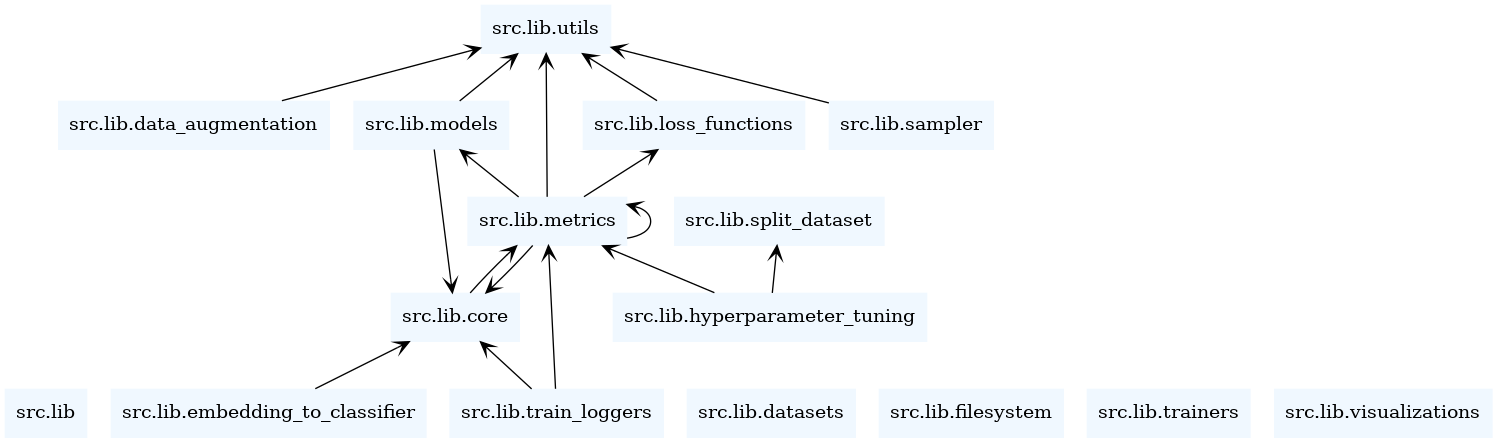
\includegraphics[width=0.8\textwidth]{informatica/diagrama_paquetes}
    \caption{Diagrama de paquetes de nuestra librería. Este diagrama ha sido creado usando la herramienta \lstinline{pyreverse}, que se ofrece como parte del programa \lstinline{pylint}.}
\end{figure}

Como deja claro el diagrama, hemos estructura el código de la librería en módulos muy interconectados entre ellos. Comentamos ahora el \textbf{propósito de los módulos más relevantes}:

\begin{itemize}
    \item \lstinline{src.lib.utils} contiene funciones auxiliares que se usan en distintas partes del código. Por ejemplo, comprobar si un tensor de \lstinline{pytorch} representa un vector o una matriz, realizar ciertos pre-cómputos para acelerar la ejecución de módulos, autentificarse en el servicio de logging \lstinline{wandb}, \ldots
    \item \lstinline{src.lib.loss_functions} contiene todo el código para computar las distintas funciones de pérdida que hemos introducido en \customref{ich:fundamentos_teoricos}.
    \item \lstinline{src.lib.sampler} contiene el código que implementa el \textit{P-K sampling}
    \item \lstinline{src.lib.metrics} implementa todas las métricas que hemos introducido en \customref{isec:metricas_teoria}
    \item \lstinline{src.lib.train_loggers} contiene la lógica para mostrar las métricas deseadas durante el ciclo de entrenamiento de forma cómoda, modular y extensible, como comentaremos en \customref{isec:loggin_metricas}
    \item \lstinline{src.lib.datasets} contiene la lógica para descargar, extraer, y cargar en una clase accesible para \lstinline{pytorch} los \textit{datasets} \textit{FG-Net} y \textit{CACD}

    \item \lstinline{src.lib.hyperparameter_tuning} contiene el código necesario para realizar \textit{hyperparameter tuning} usando \textit{K-Fold Cross Validation}
    \todo{Hacer aquí una referencia a esta técnica. Igual debería ir en la parte de teoría}

    \item \lstinline{src.lib.split_dataset} contiene el código para dividir un \textit{dataset} en dos porciones, usando dos técnicas distintas. La primera técnica consiste en separar el \textit{dataset} usando muestreo aleatorio. La segunda técnica consiste en realizar la separación usando muestreo aleatorio, pero asegurando que no existan individuos de una clase en ambos \textit{datasets} simultáneamente
    \item \lstinline{src.lib.data_augmentation} implementa el aumento de datos. Este aumento de datos es necesario porque, como hemos comentado en \customref{isubsubs:observaciones_conclusiones_pksampling}, para realizar \textit{P-K sampling} es obligatorio que todos los individuos tengan al menos $K$ imágenes asociadas. Realizamos el aumento de datos de forma clásica, añadiendo nuevos elementos a nuestro \textit{dataset}, y de forma \textit{lazy} o perezosa. En el aumento de datos \textit{lazy} no generamos nuevos elementos hasta que estos se solicitan en alguna parte del código. En \customref{isec:aumentado_datos} explicamos esto en detalle
\end{itemize}

Por la gran extensión de la base de código, mostrar el diagrama de clases completo no aporta apenas información. Pero mostraremos los diagramas de clase de ciertos módulos en \customref{isec:modulos_relevantes}, cuando esto aporte información relevante.

\section{Módulos relevantes} \label{isec:modulos_relevantes}

Por la extensión del proyecto no comentaremos cada módulo de código desarrollado. Sin embargo, en esta sección, estudiaremos algunos de los módulos más relevantes introducidos en \customref{isec:estructura_paquetes_modulos}.

\subsection{\textit{P-K sampling}}

\subsection{Aumentado de datos} \label{isec:aumentado_datos}

\subsection{Implementaciones propias de \textit{Datasets}} \label{isec:datasets_customs}

\subsection{Normalización}

Esto se usa en \cite{informatica:facenet}

\subsection{\textit{Hyperparameter Tuning}} \label{isec:hp_tuning}

\subsection{Separación de datos teniendo en cuenta obtener clases disjuntas}

\subsection{Logging de métricas} \label{isec:loggin_metricas}

wandb

\subsection{Gestion de parámetros globales en un diccionario}

Quizás hablar de ello en logging de métricas


\section{Optimización del código} \label{isec:optimizacion_codigo}

\section{Pipeline} \label{isec:pipeline}

\section{\textit{Suite} de \textit{tests}} \label{isec:test_suite}

